\documentclass[11pt,a4paper]{article}

% --- Encoding & Sprache ---
\usepackage[T1]{fontenc}
\usepackage[utf8]{inputenc}
\usepackage[ngerman]{babel}

% --- Layout & Typografie ---
\usepackage[a4paper,margin=1.5cm]{geometry} % Schmaler Rand
\usepackage{setspace}
\usepackage{enumitem}
\usepackage{hyperref}
\usepackage{graphicx}
\usepackage{array}
\usepackage{booktabs}
\usepackage{fancyhdr}
\usepackage{xcolor}
\usepackage{csquotes}
\usepackage{float}
\usepackage{placeins}

% --- Hyperref Setup ---
\hypersetup{
  pdftitle={HopIn Temporäre Event-Gruppen (HCD A5B)},
  pdfauthor={Kevin Forter, Benjamin Feichtlbauer},
  pdfsubject={Prototyp-Dokumentation},
  pdfkeywords={HCD, Prototyp, Event-Organisation, temporäre Gruppen},
  colorlinks=true,
  linkcolor=black,
  urlcolor=blue,
  citecolor=black
}

% --- Header / Footer ---
\pagestyle{fancy}
\fancyhf{}
\lhead{Studiengang: HCD}
\chead{HopIn Prototyp}
\rhead{Assignment: A5B}
\lfoot{Kevin Forter \& Benjamin Feichtlbauer}
\rfoot{\thepage}

% --- Absätze & Listen ---
\setlength{\parskip}{6pt}
\setlength{\parindent}{0pt}
\setlist[itemize]{leftmargin=1.2em}
\setlist[enumerate]{leftmargin=1.4em}

% --- Nützliche Makros ---
\newcommand{\appname}{\textbf{HopIn}}

\begin{document}

% --- Titelseite ---
\begin{titlepage}
  \centering
  {\Large Human-Centered Design (HCD)}\\[2ex]
  {\large Assignment A5B}\\[10ex]
  {\huge \textbf{HopIn}: Temporäre Event-Gruppen}\\[3ex]
  {\large Prototyp Zielsetzung, Personas und Dokumentation}\\[8ex]

  % --- Bild zentral einfügen ---
  \includegraphics[width=0.6\textwidth]{images/iphone-14-pro-mockup.png}\\[8ex]

  % --- Tabellenbereich ---
  \begin{tabular}{@{}p{4cm}p{9cm}@{}}
    \textbf{Studiengang:} & HCD \\
    \textbf{Kurs / Studierende:} & Kevin Forter \& Benjamin Feichtlbauer \\
  \end{tabular}

  \vfill
\end{titlepage}

% Inhaltsverzeichnis
\tableofcontents
\newpage

\section{Projektidee}
\appname{} ist eine mobile App (bzw.\ Web-App), mit der Nutzer temporäre Gruppen für Events erstellen können, zum Beispiel für Partys, Ausflüge, Sporttreffen oder Uni-Projekte.
Im Gegensatz zu klassischen Messenger-Gruppen wie WhatsApp, die nach dem Event bestehen bleiben, werden Gruppen bei \appname{} automatisch archiviert, sobald das Event endet.
So bleibt der Kommunikationsbereich aufgeräumt, übersichtlich und fokussiert auf das Wesentliche: gemeinsam planen, durchführen und abschließen.

\section{Zielsetzung}
Das Ziel von \appname{} ist es, die kurzfristige Event-Organisation zu vereinfachen und gleichzeitig digitale Ordnung zu fördern.
Nutzer sollen schnell Gruppen erstellen, andere einfach einladen (per Link oder QR-Code) und alle relevanten Informationen wie Chat, To-Dos und Umfragen an einem Ort bündeln können.
Nach Ende des Events verschwindet die Gruppe automatisch aus der aktiven Ansicht, bleibt aber im Archiv zur Einsicht erhalten.

\section{Zielgruppe und Ziele des Prototyps (Use Cases)}
\textbf{Zielgruppe:} Personen, die häufig spontane oder kurzfristig planbare Anlässe organisieren (Studierende, Berufstätige, Elternvertretungen) und dabei klare, temporäre Kommunikationsräume bevorzugen.

\textbf{Ziele des Prototyps:}
\begin{itemize}
  \item Schnelle Erstellung temporärer Event-Gruppen mit Titel, Datum/Uhrzeit und optionalen Rollen.
  \item Reibungsloses Einladen via Link oder QR-Code ohne Nummernspeicherung.
  \item Bündelung relevanter Funktionen: Chat, To-Dos (wer bringt was?), Umfragen (Termin/Ort) und Dateien.
  \item Automatisches Archivieren der Gruppe nach Event-Ende, weiterhin lesender Zugriff im Archiv.
  \item Übersicht über bevorstehende, laufende und archivierte Events.
\end{itemize}

\section{Persona 1: Lisa Sommer (21) Studentin}
\textbf{Beschreibung:} Lisa studiert Medienwissenschaften, wohnt in einer WG und organisiert oft spontane WG-Partys oder kleine Geburtstagsrunden. Sie hasst es, ständig neue WhatsApp-Gruppen zu erstellen, die danach nie wieder genutzt werden.

\textbf{Ziele:}
\begin{itemize}
  \item Events unkompliziert planen
  \item Leute einfach einladen (ohne Nummern zu speichern)
  \item Ordnung in ihren Kommunikations-Apps behalten
\end{itemize}

\textbf{Pain Points:}
\begin{itemize}
  \item Unübersichtliche WhatsApp-Gruppen
  \item Alte Gruppen bleiben bestehen
  \item Planungstools sind oft zu kompliziert
\end{itemize}

\textbf{User Story:}
\begin{quote}
Als Studentin möchte ich für meine WG-Party schnell eine temporäre Gruppe erstellen können, damit ich alle Gäste koordinieren kann und die Gruppe sich nach der Party automatisch archiviert, damit mein Chat wieder sauber bleibt.
\end{quote}

\section{Persona 2: Jonas Keller (28) Berufstätiger}
\textbf{Beschreibung:} Jonas ist Softwareentwickler und organisiert regelmäßig Wochenend-Aktivitäten mit Freunden, zum Beispiel Fußballspiele oder Grillabende. Er möchte die Organisation schlank und effizient halten, ohne dauerhafte Gruppen oder zu viel Chat-Spam.

\textbf{Ziele:}
\begin{itemize}
  \item Spontane Gruppen einfach erstellen
  \item Übersicht über bevorstehende Events
  \item Klare Trennung zwischen Arbeit und Freizeit
\end{itemize}

\textbf{Pain Points:}
\begin{itemize}
  \item Zu viele aktive Gruppenchats
  \item Schwer, alles im Blick zu behalten
  \item Kein einfaches Tool für kurzfristige Planung
\end{itemize}

\textbf{User Story:}
\begin{quote}
Als Berufstätiger möchte ich temporäre Gruppen für Freizeitaktivitäten erstellen können, um Termine und Aufgaben (zum Beispiel wer bringt was mit?) zu organisieren und danach automatisch alles ins Archiv verschieben lassen, damit ich nicht alles manuell löschen muss.
\end{quote}

\section{Persona 3: Sarah Baumann (35) Mutter und Elternbeirätin}
\textbf{Beschreibung:} Sarah koordiniert Schulaktivitäten, Ausflüge und Elternabende. Sie nutzt WhatsApp-Gruppen, aber es wird schnell chaotisch, wenn für jedes Event eine neue Gruppe bleibt.

\textbf{Ziele:}
\begin{itemize}
  \item Übersicht über vergangene und kommende Schul-Events
  \item Einfache Kommunikation mit anderen Eltern
  \item Strukturiertes Planen ohne Informationsverlust
\end{itemize}

\textbf{Pain Points:}
\begin{itemize}
  \item Alte Gruppen bleiben bestehen
  \item Teilnehmer vergessen, Gruppen zu verlassen
  \item Zu viele Chats ohne klare Struktur
\end{itemize}

\textbf{User Story:}
\begin{quote}
Als Elternbeirätin möchte ich für jedes Schulfest eine temporäre Gruppe erstellen können, damit ich Einladungen, Aufgaben und Infos teilen kann und nach dem Event die Gruppe automatisch archiviert wird, um Ordnung zu behalten.
\end{quote}

\section{Dokumentation des Prototyps}
\subsection{Beschreibung}
Der vorliegende Klick- und UI-Prototyp demonstriert den Kernfluss:
\begin{enumerate}
  \item Event anlegen: Titel, Datum/Zeit, Ort, Beschreibung.
  \item Einladen: Link oder QR-Code generieren, Gastbeitritt ohne Kontaktspeicherung.
  \item Koordination: Chat, To-Do-Liste (Wer bringt was?), Umfragen (Termin/Ort) und Dateien.
  \item Abschluss: Automatisches Archivieren nach Event-Ende, lesender Zugriff im Archiv.
\end{enumerate}

\section{Frame Beschreibungen}

\subsection{Login-Screen}

\begin{table}[h!]
\centering
\renewcommand{\arraystretch}{1.3}
\begin{tabular}{@{}>{\raggedright\arraybackslash}p{7cm}@{\hspace{0.8cm}}>{\centering\arraybackslash}p{7cm}@{}}
\textbf{Login-Screen einer mobilen App:} \newline
- Begrüßungstext: „Welcome back Max!“ \newline
- Untertitel: „Today is a new day. New events. More fun.“ \newline
- Umschaltmöglichkeit zwischen \textbf{Login} und \textbf{Sign Up} \newline
- Eingabefelder: \textit{Email} und \textit{Password} \newline
- Optionen: „Remember me“ und „Forgot Password?“ \newline
- Hauptbutton: „Login in“ (schwarz, zentriert) \newline
- Alternative Logins: Google und Facebook Buttons \newline
- Hinweis: „Don't you have an account? Sign up“ (unten) &
\vspace{0pt}\includegraphics[width=7cm]{images/Login.png} \\
\end{tabular}
\caption{Login-Screen der HopIn App mit Begrüßung, Eingabefeldern und Social-Login-Optionen.}
\end{table}
\FloatBarrier
\newpage

\subsection{Home-Screen}

\begin{table}[h!]
\centering
\renewcommand{\arraystretch}{1.3}
\begin{tabular}{@{}>{\raggedright\arraybackslash}p{7cm}@{\hspace{0.8cm}}>{\centering\arraybackslash}p{7cm}@{}}
\textbf{Home-Ansicht: Upcoming Events} \newline
- Überschrift: \textbf{Upcoming} zeigt bevorstehende Events an. \newline
- Suchleiste: Für Schnellsuche von kommenden Events \newline\newline
\textbf{Erste Eventkarte (Beispiel):} \textbf{Tech Meetup} in San Francisco. \newline
  - Anzeige der verbleibenden Zeit: \textbf{2 Days}. \newline
  - Button: \textbf{Details}. \newline
  - Teilnehmeranzeige: Profilbilder + Zahl. \newline\newline
\textbf{Weitere Eventkarten (Beispiel):} \newline
  - \textbf{Beach Weekend} (Malibu Beach, 5. September 2025, Jeff) \newline
  - \textbf{Ski Trip} (Hintertuxer Gletscher, 13. Januar 2026, Josef) \newline
  - \textbf{Serena’s Birthday} (Serena’s Home, 5. September 2025, Serena) \newline
- Navigationsleiste am unteren Bildschirmrand mit Icons: \textbf{Home}, \textbf{Archive}, \textbf{Profile}. \newline\newline
Eine Eventkarte zeigt immer folgende Eigenschaften auf: \newline
- Jede Karte zeigt ein passendes Hintergrundbild zum Event. \newline
- Titel \newline
- Austragungsort \newline
- Datum \newline
- Organisator \newline
- Tage bis zum Event, Detail-Button, wie viele Personen kommen und deren Avatar (nur für oberstes Event) &
\vspace{0pt}\includegraphics[width=7cm]{images/Home.png} \\
\end{tabular}
\caption{Home-Screen der HopIn App mit Übersicht über bevorstehende Events („Upcoming“).}
\end{table}
\FloatBarrier
\newpage

\subsection{Archive-Screen}

\begin{table}[h!]
\centering
\renewcommand{\arraystretch}{1.3}
\begin{tabular}{@{}>{\raggedright\arraybackslash}p{7cm}@{\hspace{0.8cm}}>{\centering\arraybackslash}p{7cm}@{}}
\textbf{Archiv-Ansicht: Vergangene Events} \newline
- Überschrift: \textbf{Archive} mit Jahreszahl \textbf{2025}. \newline
- Suchleiste: Für Schnellsuche von kommenden Events \newline
- Filter: Filteroptionen für eine schnelle Filterung von Events ebenfalls mit Datum-Filter vorhanden \newline
- Anzeige archivierter Events in Kartenform. \newline\newline
\textbf{Erstes Event:} \textbf{Wine Tasting} \newline
  - Ort: Stadthalle \newline
  - Datum: 15. September 2025 \newline
  - Veranstalterin: Simona \newline
\textbf{Zweites Event:} \textbf{Home Party} \newline
  - Ort: Gia’s Home \newline
  - Datum: 3. August 2025 \newline
  - Veranstalterin: Gia \newline
- Navigationsleiste unten mit Icons: \textbf{Home}, \textbf{Archive} (aktiv markiert), \textbf{Profile}. \newline\newline
Eine Eventkarte zeigt immer folgende Eigenschaften auf: \newline
- Jede Karte zeigt ein passendes Hintergrundbild zum Event. \newline
- Titel \newline
- Austragungsort \newline
- Datum \newline
- Organisator &
\vspace{0pt}\includegraphics[width=7cm]{images/Archive.png} \\
\end{tabular}
\caption{Archiv-Ansicht der HopIn App mit vergangenen Events aus dem Jahr 2025.}
\end{table}
\FloatBarrier
\newpage

\subsection{Profil-Screen}

\begin{table}[h!]
\centering
\renewcommand{\arraystretch}{1.3}
\begin{tabular}{@{}>{\raggedright\arraybackslash}p{7cm}@{\hspace{0.8cm}}>{\centering\arraybackslash}p{7cm}@{}}
\textbf{Profil-Ansicht: Nutzerübersicht und Aktionen} \newline
- Überschrift: \textbf{Profile}. \newline
- Headerbild mit farbigem Hintergrundmotiv. \newline
- Profilbereich mit Avatar und Benutzerinformationen: \newline
  - Name: \textbf{Gian Müller} \newline
  - Nutzername: \texttt{@gianmüller} (kopierbar). \newline
- Aktionen unterhalb des Profils: \newline
  - \textbf{Create Event} mit Plus-Symbol. \newline
  - \textbf{Your Events} mit Kronen-Symbol. \newline
- Großer lilafarbener Button: \textbf{Logout}. \newline
- Navigationsleiste am unteren Bildschirmrand mit Icons: \textbf{Home}, \textbf{Archive}, \textbf{Profile} (aktiv markiert). \newline\newline
Ein Profil zeigt immer folgende Eigenschaften auf: \newline
- Jedes Profil zeigt ein passendes Hintergrundbild auf. \newline
- Voller Name \newline
- Benutzername \newline
- Profil Avatar &
\vspace{0pt}\includegraphics[width=7cm]{images/Profile.png} \\
\end{tabular}
\caption{Profil-Ansicht der HopIn App mit Benutzerinformationen und Aktionsmöglichkeiten.}
\end{table}
\FloatBarrier
\newpage

\subsection{Create Event, Your Events und Logout}

\begin{table}[h!]
\centering
\renewcommand{\arraystretch}{1.3}
\begin{tabular}{@{}>{\raggedright\arraybackslash}p{7cm}@{\hspace{0.8cm}}>{\centering\arraybackslash}p{7cm}@{}}
\textbf{Event erstellen – Screen:} \newline
- Titel: \textbf{Create Event}. \newline
- Bereich \textbf{Cover}: ermöglicht das Hochladen eines Event-Bildes. \newline
- Abschnitt \textbf{Details}: Eingabefelder für Name und Location. \newline
- Datums- und Zeitfelder für Start und Option mit Ende des Events. \newline
- Option \textbf{Chat Function} mit Schalter zum Aktivieren/Deaktivieren. \newline
- Option \textbf{Bring List} mit Schalter zum Aktivieren/Deaktivieren und Schalter zum hinzufügen von weiteren Items\newline
- Großer Button unten: \textbf{Create Event}. \newline
- Navigationsleiste unten: \textbf{Home}, \textbf{Archive}, \textbf{Profile} (aktiv markiert). &
\vspace{0pt}\includegraphics[width=7cm]{images/Event erstellen.png} \\
\end{tabular}
\caption{„Event erstellen“-Screen der HopIn App zum Anlegen neuer Veranstaltungen.}
\end{table}
\FloatBarrier
\newpage

\begin{table}[h!]
\centering
\renewcommand{\arraystretch}{1.3}
\begin{tabular}{@{}>{\raggedright\arraybackslash}p{7cm}@{\hspace{0.8cm}}>{\centering\arraybackslash}p{7cm}@{}}
\textbf{Your Events – Screen:} \newline
- Titel: \textbf{Your Events}. \newline
- Filter: Filteroptionen für eine schnelle Filterung von Events ebenfalls mit Datum-Filter vorhanden \newline
- Anzeige eigener Events gruppiert nach Jahr (z. B. 2025). \newline
- Beispielkarte: \textbf{Boys Trip} \newline
  - Ort: Somewhere \newline
  - Datum: 26. November 2025 \newline
  - Veranstalter: Gian \newline
  - Badge oben rechts: \textbf{Host}. \newline
- Navigationsleiste unten: \textbf{Home}, \textbf{Archive}, \textbf{Profile} (aktiv markiert). \newline\newline
Eine Eventkarte zeigt immer folgende Eigenschaften auf: \newline
- Jede Karte zeigt ein passendes Hintergrundbild zum Event. \newline
- Titel \newline
- Austragungsort \newline
- Datum \newline
- Organisator &
\vspace{0pt}\includegraphics[width=7cm]{images/Your Events.png} \\
\end{tabular}
\caption{„Your Events“-Screen der HopIn App mit Übersicht über eigene Events.}
\end{table}
\FloatBarrier
\newpage

\begin{table}[h!]
\centering
\renewcommand{\arraystretch}{1.3}
\begin{tabular}{@{}>{\raggedright\arraybackslash}p{7cm}@{\hspace{0.8cm}}>{\centering\arraybackslash}p{7cm}@{}}
\textbf{Logout-Bestätigungsdialog:} \newline
- Wird nach Betätigung des \textbf{Logout}-Buttons im Profil angezeigt. \newline
- Hintergrund des Profils ist leicht unscharf (Blur-Effekt). \newline
- Pop-up mit Text: „Are you sure you want to logout?“. \newline
- Zwei Schaltflächen: \textbf{Confirm} (zum Abmelden) und \textbf{Cancel} (zum Abbrechen). \newline
- Einheitliches Design im Stil von iOS-Systemdialogen. &
\vspace{0pt}\includegraphics[width=7cm]{images/Logout.png} \\
\end{tabular}
\caption{Logout-Dialog der HopIn App mit Bestätigung und Abbruchoption.}
\end{table}
\FloatBarrier
\newpage

\subsection{Archiviertes Event: Elternabend}

\begin{table}[h!]
\centering
\renewcommand{\arraystretch}{1.3}
\begin{tabular}{@{}>{\raggedright\arraybackslash}p{7cm}@{\hspace{0.8cm}}>{\centering\arraybackslash}p{7cm}@{}}
\textbf{Archiviertes Event – Detailansicht:} \newline
- Titel: \textbf{Archive Info}. \newline
- Großes Headerbild des Events. \newline
- Eventtitel: \textbf{Elternabend}. \newline
- Ort: \textbf{Schulhaus}. \newline
- Datum: \textbf{1. Juli 2025}. \newline
- Organisatorin: \textbf{Manuela}. \newline
- Abschnitt \textbf{Guest List}: zeigt Avatare der Teilnehmer (+5). \newline
- Abschnitt \textbf{Chat (read-only)}: zeigt einen archivierten Chatverlauf. \newline
- Chat-Beispiel: Nachrichten von „Team Unicorns“, zuletzt online vor 45 Minuten. \newline
- Navigationsleiste unten mit Icons: \textbf{Home}, \textbf{Archive} (aktiv markiert), \textbf{Profile}. &
\vspace{0pt}\includegraphics[width=7cm]{images/Elternabend.png} \\
\end{tabular}
\caption{Archivierte Event-Detailansicht „Elternabend“ mit Gästeliste und read-only Chat.}
\end{table}
\FloatBarrier
\newpage

\subsection{Event: Serena’s Birthday – Startansicht}

\begin{table}[h!]
\centering
\renewcommand{\arraystretch}{1.3}
\begin{tabular}{@{}>{\raggedright\arraybackslash}p{6.5cm}@{\hspace{0.8cm}}>{\centering\arraybackslash}p{7.5cm}@{}}
\vspace{0pt}%
\textbf{Event Info – Startansicht:} \newline
- Titel: \textbf{Event Info}. \newline
- Großes Headerbild mit Torte und Wunderkerzen. \newline
- Eventtitel: \textbf{Serena’s Birthday}. \newline
- Ort: Serena’s Home. \newline
- Datum: 5. September 2025. \newline
- Zeit: 18:00 bis Open End \newline
- Organisatorin: Serena. \newline
- Abschnitt \textbf{Guests}: Profilbilder +5. \newline
- Drei Aktionsbuttons: \textbf{Zusage (grün)}, \textbf{Absage (rot)}, \textbf{Unentschieden (blau)}. \newline
- Abschnitt \textbf{Bringlist}: Beer, Spritzer, Cake, Music Box. \newline
- Chatbutton mit zwei neuen Nachrichten (nur in diesem Beispiel vorhanden) \newline
- Navigationsleiste unten: \textbf{Home} (aktiv), Archive, Profile. \newline\newline
Ein Event zeigt immer folgende Eigenschaften auf: \newline
- Jede Karte zeigt ein passendes Hintergrundbild zum Event. \newline
- Titel \newline
- Austragungsort \newline
- Datum \newline
- Zeit \newline
- Organisator \newline
- Gästeliste mit Teilnahme Button &
\vspace{0pt}\includegraphics[width=7.5cm]{images/Birthday-3.png} \\
\end{tabular}
\caption{Startansicht des Events „Serena’s Birthday“.}
\end{table}
\FloatBarrier
\newpage

\subsection{Event: Serena’s Birthday – Teilnahme bestätigt}

\begin{table}[h!]
\centering
\renewcommand{\arraystretch}{1.3}
\begin{tabular}{@{}>{\raggedright\arraybackslash}p{6.5cm}@{\hspace{0.8cm}}>{\centering\arraybackslash}p{7.5cm}@{}}
\textbf{Event Info – Teilnahme bestätigt:} \newline
- Gleiche Ansicht wie Startbildschirm. \newline
- Grüner Button (Zusage) aktiviert. \newline
- Gästezahl erhöht sich auf \textbf{+6}. \newline
- Zeigt, dass der Benutzer die Teilnahme zugesagt hat. \newline
- Alle weiteren Informationen identisch zur Startansicht. &
\vspace{0pt}\includegraphics[width=7.5cm]{images/Birthday-1.png} \\
\end{tabular}
\caption{Event „Serena’s Birthday“ – Teilnahme bestätigt.}
\end{table}
\FloatBarrier
\newpage

\subsection{Event: Serena’s Birthday – Teilnahme abgelehnt}

\begin{table}[h!]
\centering
\renewcommand{\arraystretch}{1.3}
\begin{tabular}{@{}>{\raggedright\arraybackslash}p{6.5cm}@{\hspace{0.8cm}}>{\centering\arraybackslash}p{7.5cm}@{}}
\textbf{Event Info – Teilnahme abgelehnt:} \newline
- Gleiche Grundstruktur wie Startansicht. \newline
- Roter Button (Absage) aktiviert. \newline
- Gästezahl zurück auf \textbf{+5}. \newline
- Event bleibt sichtbar, jedoch markiert als abgelehnt. \newline
- Bringlist und Gästeübersicht weiterhin sichtbar. &
\vspace{0pt}\includegraphics[width=7.5cm]{images/Birthday-2.png} \\
\end{tabular}
\caption{Event „Serena’s Birthday“ – Teilnahme abgelehnt.}
\end{table}
\FloatBarrier
\newpage

\subsection{Event: Serena’s Birthday – Teilen per QR-Code}

\begin{table}[h!]
\centering
\renewcommand{\arraystretch}{1.3}
\begin{tabular}{@{}>{\raggedright\arraybackslash}p{6.5cm}@{\hspace{0.8cm}}>{\centering\arraybackslash}p{7.5cm}@{}}
\textbf{Event teilen – QR-Code-Ansicht:} \newline
- Pop-up im Ticket-Stil mit QR-Code zur Einladung. \newline
- Titel: \textbf{Serena’s Birthday by Serena}. \newline
- Anzeige von Start- und Endzeit: 05.09.25 (18:00) – Open End. \newline
- Hinweis: „Scan the QR-Code to enter the group“. \newline
- Unten: sechsstelliger Beitrittscode mit Kopier-Icon. \newline
- Hintergrund leicht unscharf (Blur-Effekt). \newline\newline
Eine Sharecard zeigt immer folgende Eigenschaften auf: \newline
- Jede Karte zeigt einen passenden QR-Code zum Event. \newline
- Titel \newline
- Organisator \newline
- Start-Datum \newline
- Start-Zeit \newline
- End-Datum \newline
- End-Zeit \newline
- Gästeliste mit Teilnahme Button &
\vspace{0pt}\includegraphics[width=7.5cm]{images/Birthday-Share.png} \\
\end{tabular}
\caption{Event „Serena’s Birthday“ – Teilen über QR-Code-Einladung.}
\end{table}
\FloatBarrier
\newpage

\subsection{Event: Serena’s Birthday – Chatansicht}

\begin{table}[h!]
\centering
\renewcommand{\arraystretch}{1.3}
\begin{tabular}{@{}>{\raggedright\arraybackslash}p{6.5cm}@{\hspace{0.8cm}}>{\centering\arraybackslash}p{7.5cm}@{}}
\vspace{0pt}%
\textbf{Chatansicht des Events „Serena’s Birthday“:} \newline
- Titel: \textbf{Chat}. \newline
- Chatgruppe: \textbf{Team Unicorns}. \newline
- Anzeige des letzten Online-Status: „last seen 45 minutes ago“. \newline
- Avatare der Gruppenmitglieder in der Kopfzeile. \newline
- Nachrichten chronologisch sortiert (z. B. 18 October 2025). \newline
- Unterschiedliche Rollen und Namen: Jav (Engineering), Aubrey (Product), Janet (Engineering/Product). \newline
- Nachrichtenverlauf: Unterhaltung über Lunch-Pläne. \newline
- Nachrichten des Nutzers in blauen Sprechblasen (rechts), andere Teilnehmer in grauen (links). \newline
- Eingabefeld unten mit Text „Start typing…“ und Symbolen für Emoji und Senden. &
\vspace{0pt}\includegraphics[width=7.5cm]{images/Chat.png} \\
\end{tabular}
\caption{Chatansicht des Events „Serena’s Birthday“ mit Gruppengespräch und Rollenkennzeichnung.}
\end{table}
\FloatBarrier
\newpage

\subsection{Event: Serena’s Birthday – Album}

\begin{table}[h!]
\centering
\renewcommand{\arraystretch}{1.3}
\begin{tabular}{@{}>{\raggedright\arraybackslash}p{6.5cm}@{\hspace{0.8cm}}>{\centering\arraybackslash}p{7.5cm}@{}}
\vspace{0pt}%
\textbf{Album-Ansicht des Events:} \newline
- Titel in der Kopfzeile: \textbf{Album} mit Zurück-Navigation. \newline
- Rasterdarstellung vieler Fotos (gleich große Thumbnails in Spalten und Zeilen). \newline
- Bilder stammen aus dem Event \textit{Serena’s Birthday}. \newline
- Jedes Bild zeigt eine Szene vom gleichen Ort (Strandmotiv). \newline
- Untere Navigationsleiste mit \textbf{Home} (aktiv), \textbf{Archive}, \textbf{Profile}. \newline
- Dient der schnellen visuellen Übersicht aller im Event geteilten Medien. &
\vspace{0pt}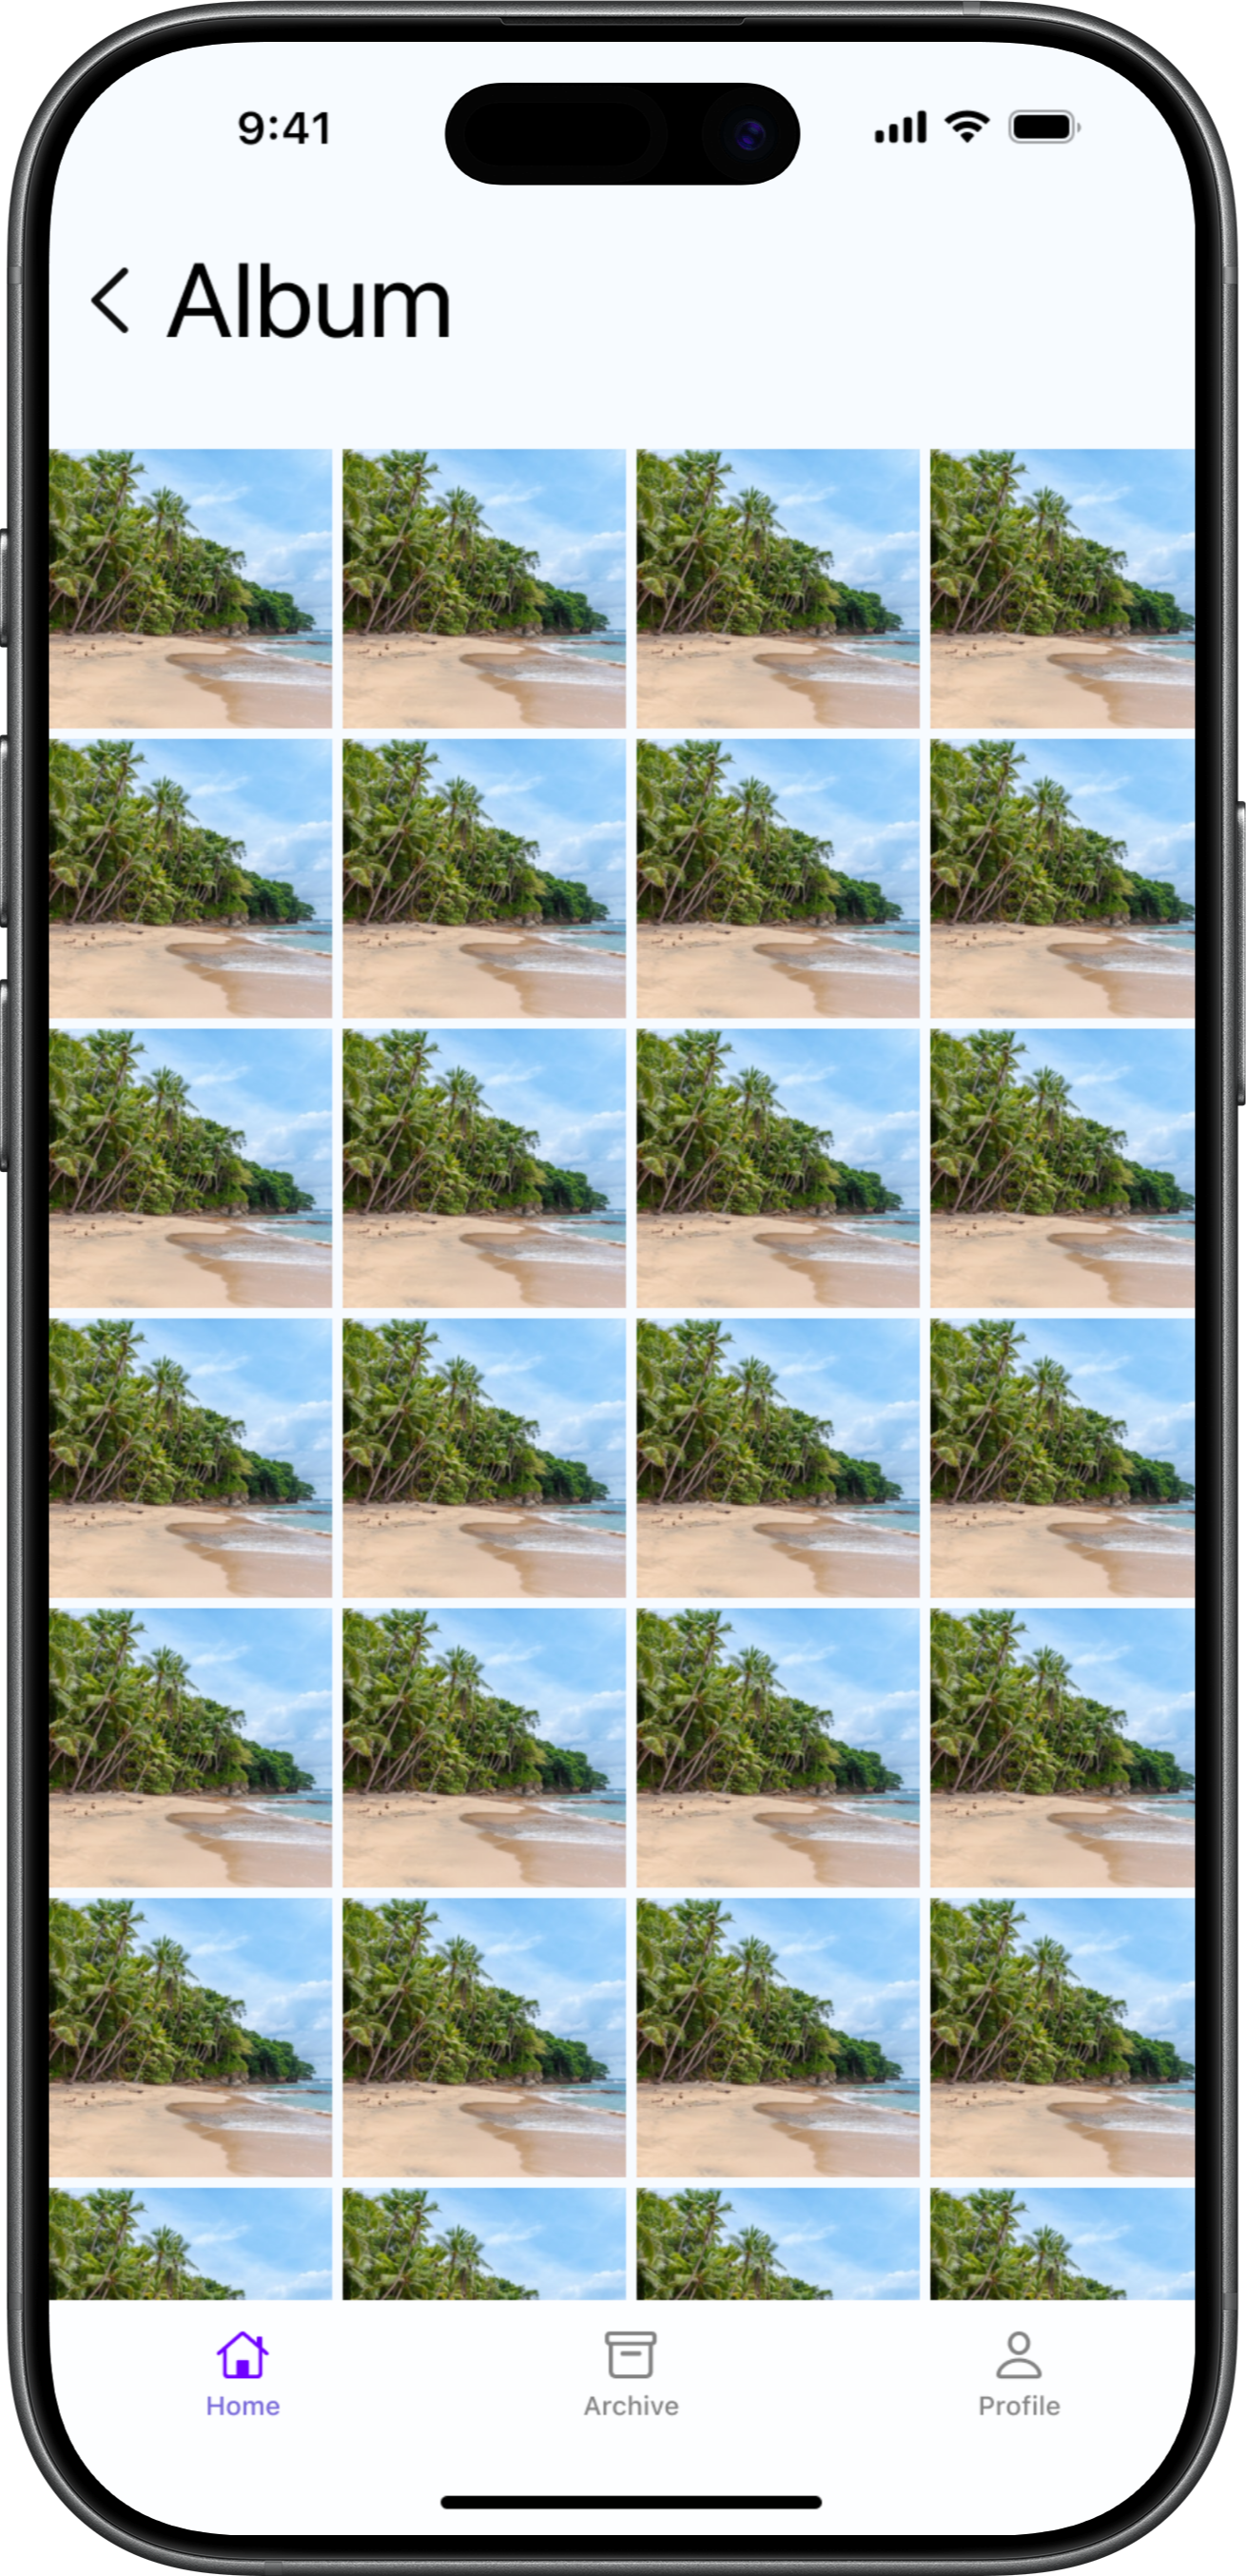
\includegraphics[width=7.5cm]{images/Album.png} \\
\end{tabular}
\caption{Album-Ansicht der im Event „Serena’s Birthday“ geteilten Bilder.}
\end{table}
\FloatBarrier
\newpage

\section{User Flow Diagramm}

\begin{figure}[h!]
  \centering
  \includegraphics[width=\textwidth]{images/userflow.png}
  \caption{User Flow des HopIn-Prototyps}
\end{figure}
\FloatBarrier

Der gezeigte \textbf{User Flow} visualisiert die gesamte Nutzerinteraktion innerhalb der \appname{} App – 
vom Start bis hin zu den Event-Details und der Profilverwaltung. Nach dem App-Start wird geprüft, 
ob der Benutzer bereits eingeloggt ist. Ist dies nicht der Fall, gelangt er zunächst zum \textbf{Login}-Screen. 
Nach erfolgreichem Login öffnet sich die \textbf{Home-Ansicht} mit allen anstehenden Events (\textit{Upcoming}).

Von dort aus führen Tabs zu den drei Hauptbereichen:
\begin{itemize}
  \item \textbf{Home:} Zugriff auf Event-Details, Zusage/Ablehnung, Teilen per QR-Code, Chat und Album-Ansicht.
  \item \textbf{Archive:} Zugriff auf vergangene, archivierte Events im Lesemodus (\textit{read-only}).
  \item \textbf{Profile:} Verwaltung eigener Events (Erstellen, Anzeigen) sowie Logout-Funktion.
\end{itemize}

Jeder Bereich ist miteinander verknüpft und über die untere Navigationsleiste erreichbar.
Der Flow zeigt somit den vollständigen Interaktionspfad eines typischen Nutzers innerhalb der Anwendung – 
von der Event-Erstellung bis zur Archivierung.

\newpage
\section{Figma Prototyp – Gesamtübersicht}

\begin{figure}[h!]
  \centering
  \includegraphics[width=\textwidth]{images/Figma.png}
  \caption{Gesamtübersicht des Figma-Prototyps}
\end{figure}
\FloatBarrier

Die Abbildung zeigt den vollständigen \textbf{Figma-Prototyp} der \appname{}-App in seiner strukturellen Übersicht. 
Die zuvor dargestellten Screens stellen dabei nur einen kleinen Ausschnitt der gesamten Anwendung dar.  
Jedes Event im System ist individuell aufrufbar und besitzt seinen eigenen Frame mit spezifischen Ansichten 
(z.\,B.\ Event-Info, Chat, Bringlist, QR-Code oder Album).  

Auch archivierte Events verfügen über eigene Frames, die eine \textit{read-only}-Darstellung der Inhalte bieten.  
Die umfangreiche Prototypen-Struktur verdeutlicht die hohe Interaktivität und die vollständige Abbildung des 
Nutzerflusses – von der Anmeldung über Event-Erstellung bis hin zur Archivierung vergangener Veranstaltungen.

\newpage
\section{Logo Beschreibung}

Das Logo von \textbf{HopIn} besteht aus einer minimalistischen, geometrischen Form, die aus verbundenen Linien in einem sanften Violett-Ton gestaltet ist. Die klaren Linien und sechseckigen Elemente symbolisieren Struktur, Verbindung und Dynamik – zentrale Werte der App.

\textbf{Bedeutung für das Projekt:}
Das Logo visualisiert die Idee von \textit{temporären Verbindungen}. Ähnlich wie die App selbst vernetzt es einzelne Punkte zu einer klaren, temporären Struktur. Die offene, lineare Form vermittelt Flexibilität und Einfachheit, während die Farbwahl in Violett Modernität und Kreativität ausdrückt.  
Die Kombination aus Struktur und Bewegung steht für das Prinzip von HopIn: \textit{Gruppen bilden sich, funktionieren effizient – und lösen sich nach dem Event elegant wieder auf.}

\begin{center}
    \includegraphics[width=\textwidth]{images/logo.png}
\end{center}

\section{Link (mit Bearbeitungszugriff)}
\textbf{Prototyp-URL:}  
\url{https://www.figma.com/file/Dmgm18zgv7DBHrGzGCSv53?node-id=3:3&locale=de&type=design}

\vfill
\textit{Erstellt von:} Kevin Forter \& Benjamin Feichtlbauer

\end{document}